% CREATED BY MAGNUS GUSTAVER, 2020
\chapter{Results}
This results in this chapter are based on the validation assessments outlined in Sec.~\ref{sec:val}. It includes paragraphs and figures detailing the updated graphical user interface, flight control process, and object detection. 

\section{Graphical User Interface}\label{res: GUI}
The updated GUI was incorporated, which included several additional buttons, while still maintaining the same general layout as depicted in Fig.~\ref{fig:GUI_v1}. The objective was to ensure that the GUI fulfilled specific requirements, such as user-friendliness, visual hierarchy, real-time presentation, and inclusion of all necessary commands. To achieve this, the application employed a single activity that displayed all information on the screen. This design helped users avoid the hassle of navigating through various activities and accidentally pressing the wrong buttons. Furthermore, since the mobile device was connected to the controller in landscape mode, the application was locked to this orientation.
\newline
\begin{figure}[!h]
    \centering
    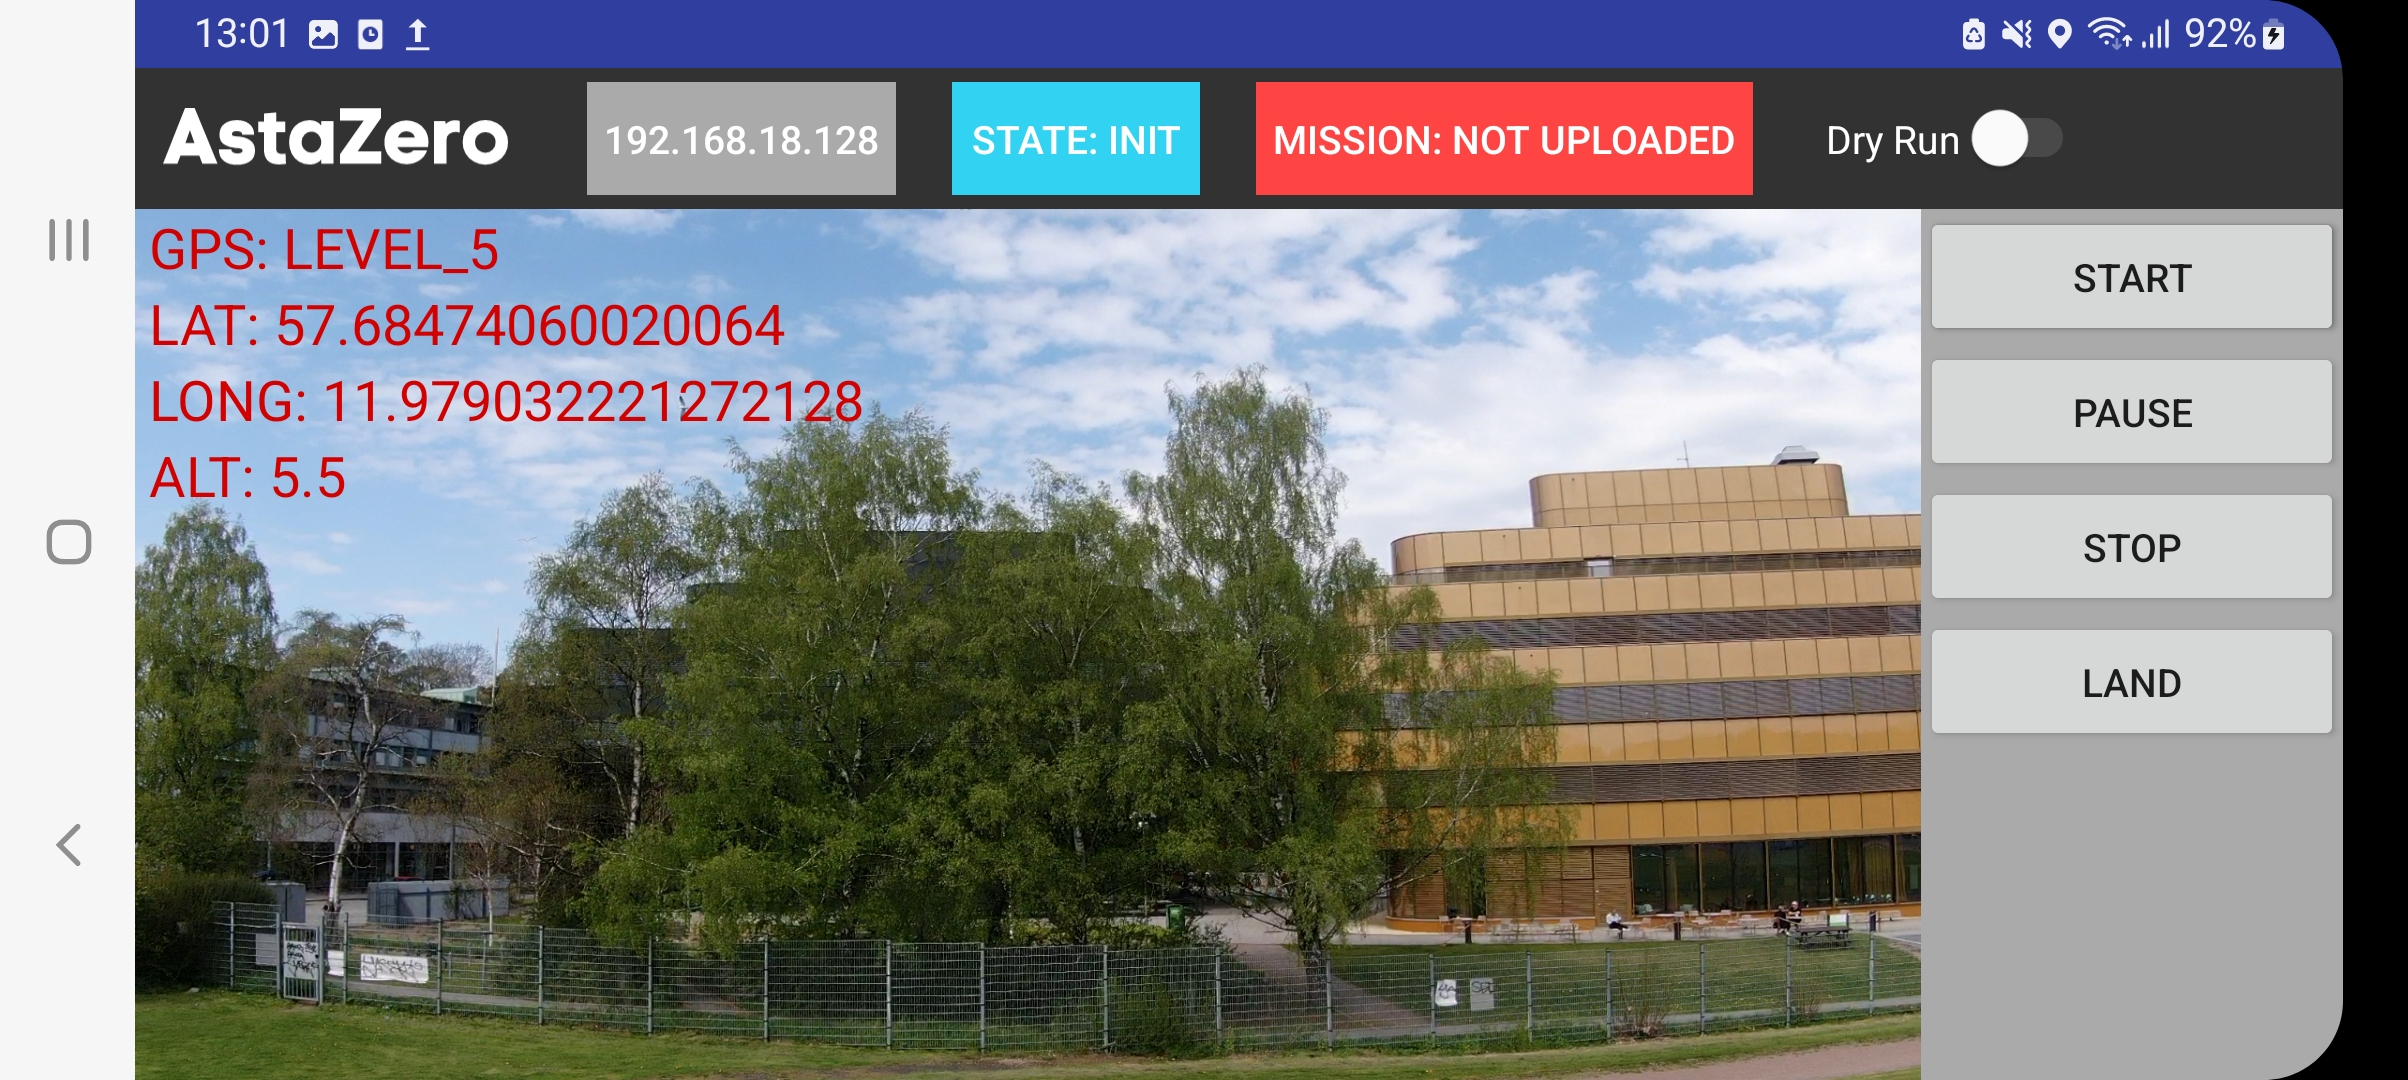
\includegraphics[width=1\textwidth]{figure/gui_klar.jpg}
    \caption{GUI visualization while flying manual flight. Source: Primary}
    \label{fig:gui_klar}
\end{figure}

In the left center of the screen, the live video feed from the drone can be found, catching the user's attention as it is the main focus of the program. The less relevant data, such as longitudinal and latitudinal coordinates, as well as GPS and altitude, is displayed above the video feed in red to make it stand out. This information constantly changes and is only relevant if the program needs to be debugged. The header consists of three different text boxes and a slider button, showing vital information to the operator. ATOS works with IP addresses to connect to different test objects and therefore it is relevant to show which IP address the drone currently possesses. The state of the drone is shown in the middle text box with visual information being given in both text and color, shown in Fig.~\ref{fig:gui_klar}, Fig.~\ref{fig:gui_disarmed_traj} and Fig.~\ref{fig:gui_running_fail}. Depending on what state the drone is in, the text box will change color according to the same color scheme used in the ATOS control interface. This gives a quick and clear indication if the drone is in the intended state. Similarly, the third text box also changes color depending on what state WaypointMission currently is  in. When uploading the mission, it changes to cyan and switches to green when the mission is executing. \newline
\begin{figure}[!h]
    \centering
    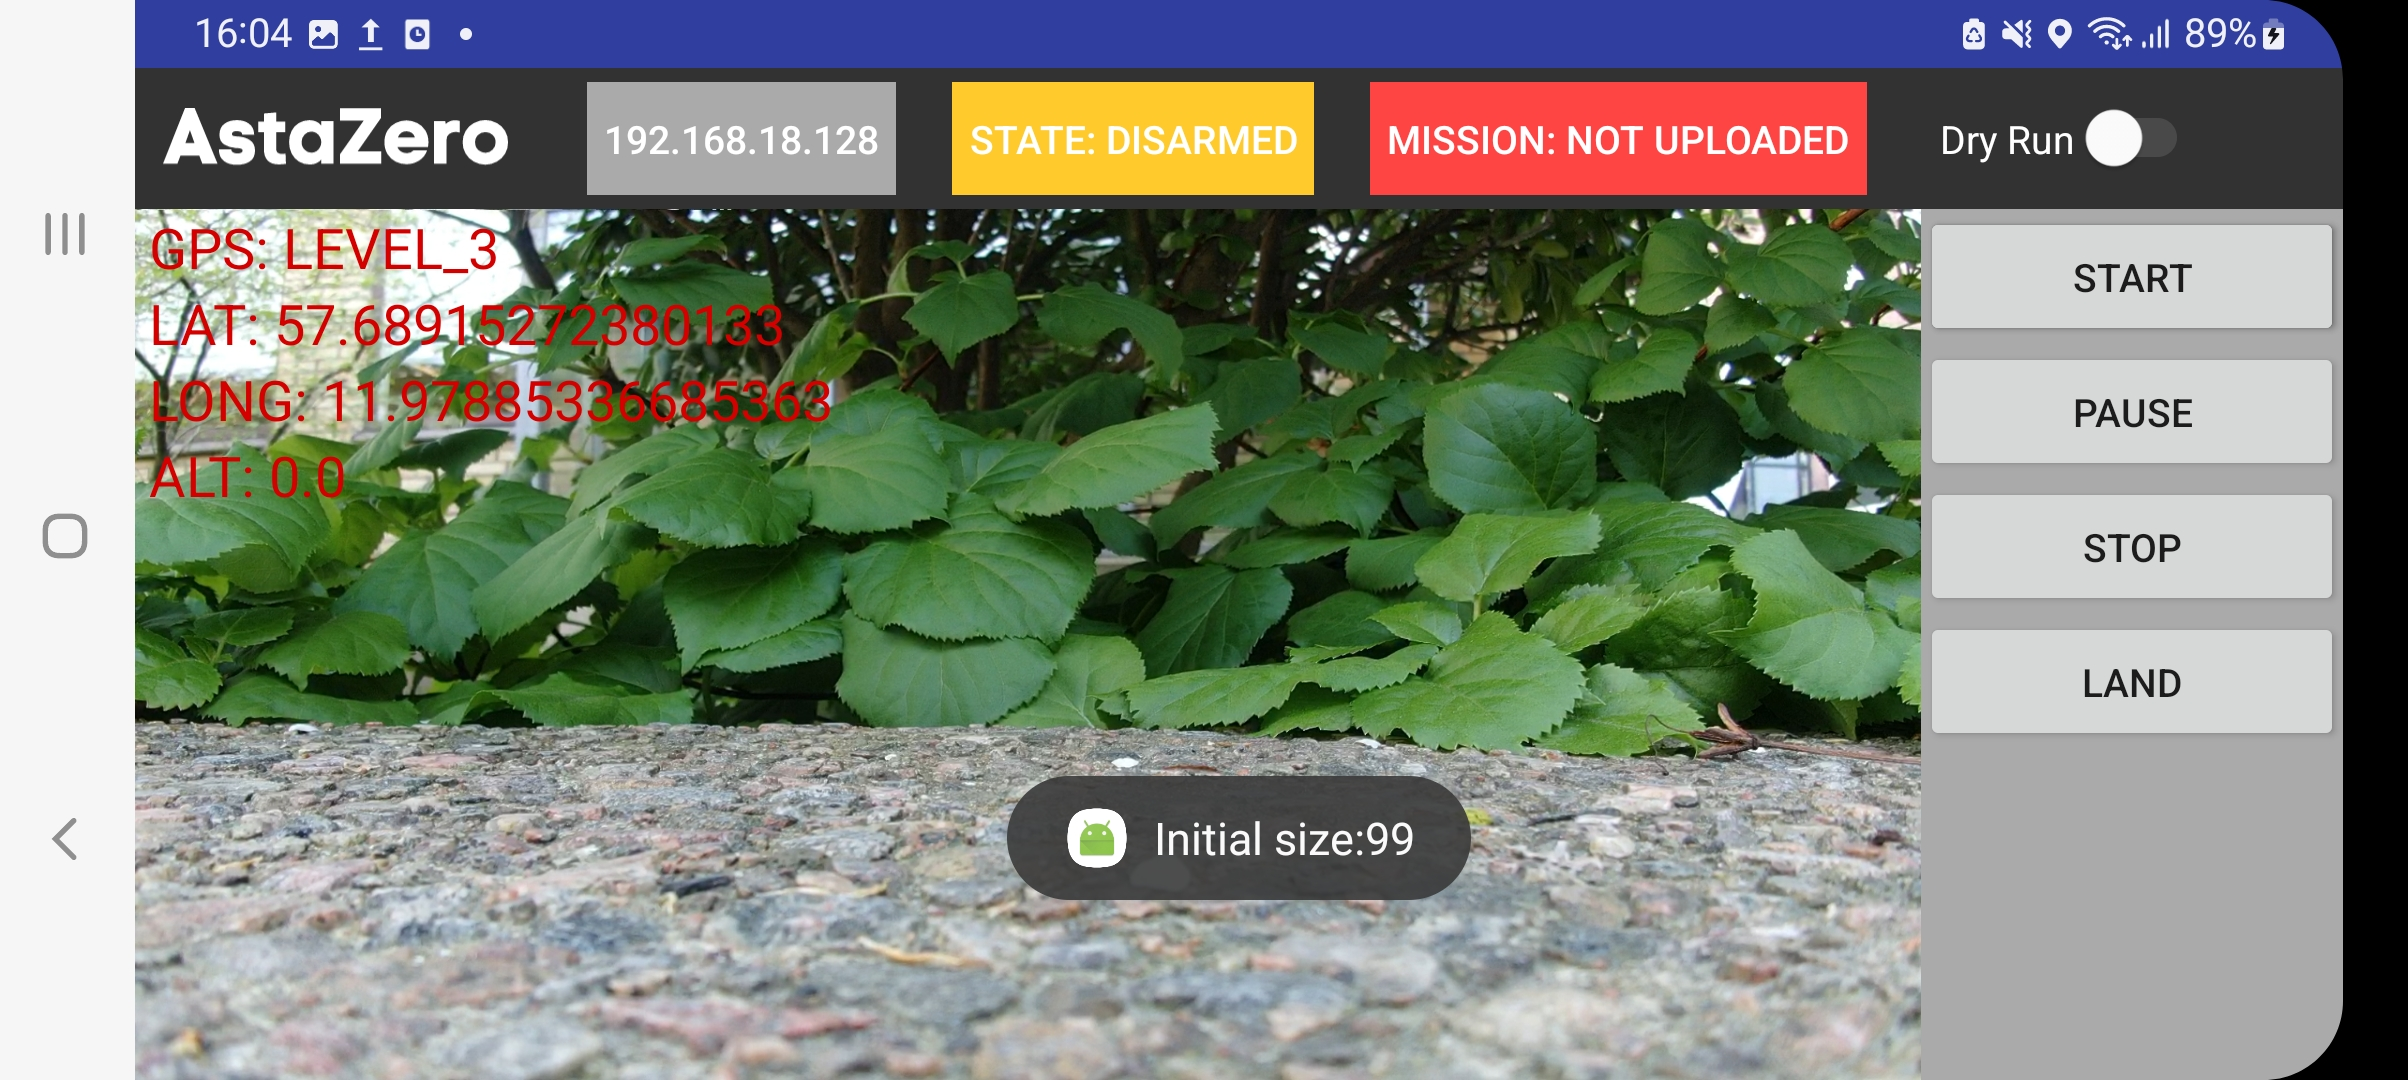
\includegraphics[width=1\textwidth]{figure/gui_disarmed_traj.jpg}
    \caption{GUI when in the ''Disarmed'' state and receiving trajectory. Source: Primary}
    \label{fig:gui_disarmed_traj}
\end{figure}

There is also an indication of how many waypoints the mission consists of and what waypoint the drone is currently heading to or currently uploading, as shown in Fig.~\ref{fig:gui_running_fail}. As also shown in the figure, if the drone has not completed all steps and is ready for the running phase, the GUI will show an error message and not execute the mission. The ``Dry run'' slider enables the operator to decide if the drone should be part of the test or not. The slider is not changeable when a test is executing, it can only be switched when the drone is in the ``Disarmed'' or ``Armed'' modes. 
\begin{figure}[h!]
    \centering
    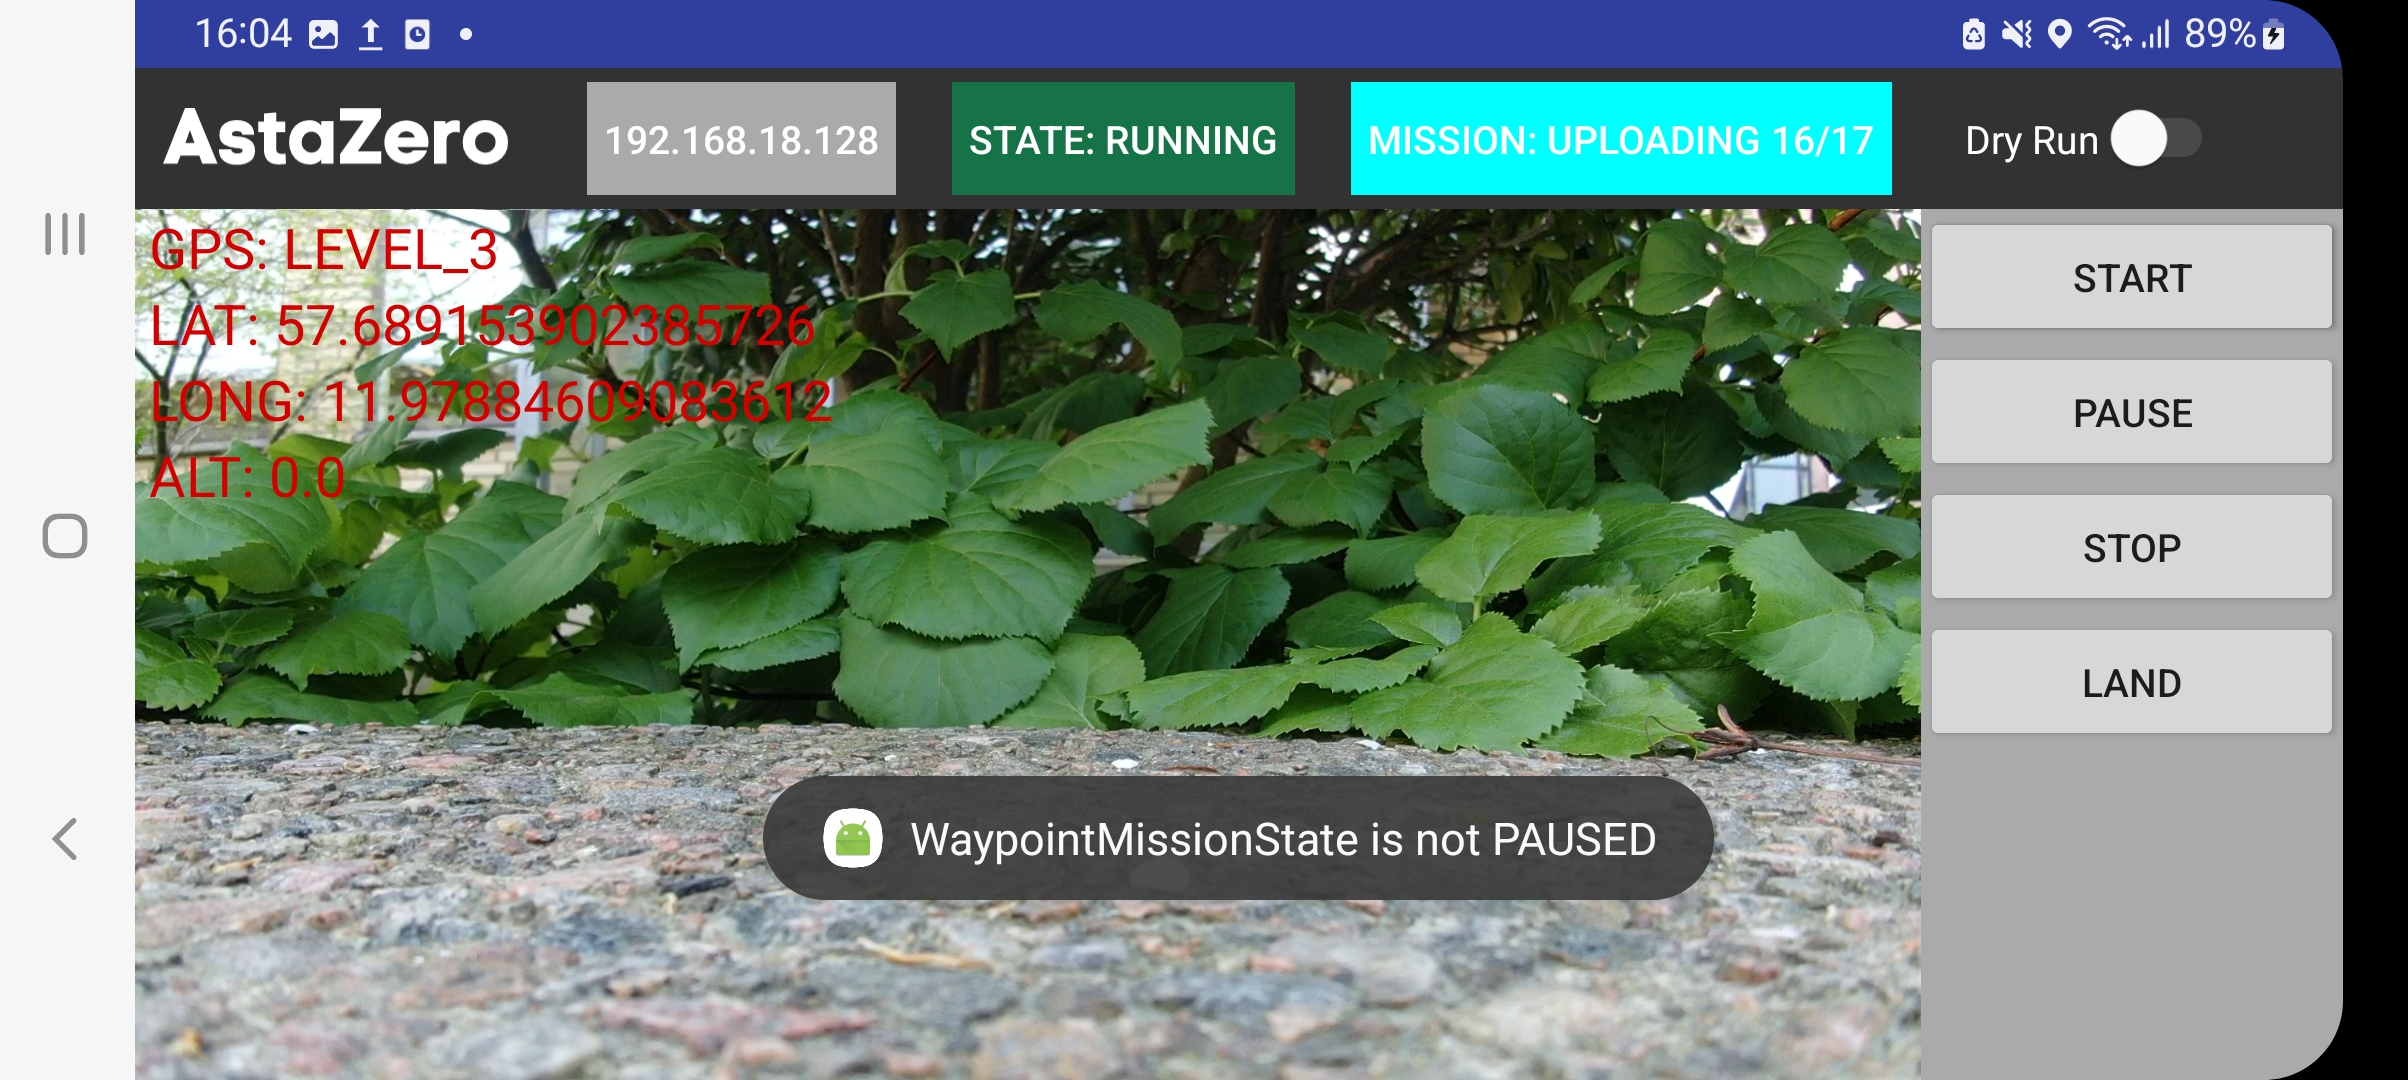
\includegraphics[width=1\textwidth]{figure/gui_running_fail.jpg}
    \caption{GUI when the drone is in the ''Running'' state and has not finished uploaded all waypoints. Source: Primary}
    \label{fig:gui_running_fail}
\end{figure}
\\ \\
The buttons added on the right-hand side are responsible for controlling the functionality of the drone, including initiating an uploaded WaypointMission, pausing it, stopping it, and landing. This provides an efficient means for an operator to promptly halt a mission if any anomalies are detected or if an emergency arises. Moreover, it facilitates developers' interaction with the application while testing new features, ensuring that the drone can always be halted and landed if necessary.
\section{Flight control} \label{res:FLIGHT}

The foundation for the flight control, as outlined in Sec.~\ref{sec:val_flight}, paved the way for the drone to run the desired Euro NCAP tests via ATOS. To do this, the drone must first connect to the ATOS server. As the application handles the ISO-object in the background, establishing the connection is relatively simple. All that is needed is to ensure that the server device and the mobile device are on the same network, configure the relevant files, and provide ATOS with the IP address of the mobile device. Once ATOS starts running, it will automatically connect to the given IP address and begin communicating with the ISO-object in each test object via the ISO DTS 22133 protocol mentioned in Sec.~\ref{ISO}. When the connection is established, all test objects can be initiated and their states switched to ``Disarmed'' upon connection to ATOS.\newline

After establishing a connection with ATOS and the drone, the application can receive trajectories, modify, convert and deploy them to the drone. If the trajectories consist of too many points, they will be correctly reduced by Algorithm \ref{DP_code}. A small popup window on the mobile device screen will show the number of waypoints in the trajectory prior to reduction, and another popup will indicate the number of waypoints remaining after the reduction. The application then converts the trajectories from the ATOS format to the DJI WaypointMission format, preparing them for deployment to the drone. 
\newline

% positioning at ARMED
Upon initiation of ATOS and the transition from the ``Init'' state to the ``Armed'' state, the flight path is able to be uploaded to the drone, and afterward take off autonomously. The drone will then ascend to an altitude specified within ATOS, and proceeded towards the test origin where the first waypoint is located. This procedure was thoroughly tested from multiple positions surrounding the test origin, and the drone consistently arrived at the origin, awaiting the ``Run'' command of the test before executing the remainder of the mission.
\newline

% starting mission
Once ATOS transitions all test objects to the ``Running'' state, the Android application issues a command to resume the paused WaypointMission and from a hovering position, the drone proceeds to execute the remaining waypoints on the  flight path. Throughout all states of the test, the Android application continuously updates the GUI with all relevant information, as described in the previous section. When the mission is finished, the application is capable of autonomously flying the drone back to the position from where it took off.   
\newline  

In summary, the drone has the ability to autonomously take off, navigate its flight path, and land with precision. All of this is achieved and managed through ATOS, without requiring any external input to correctly execute the supplied trajectories at the right time. 

\section{Object detection and tracking} \label{res:OBJECT}
The current version of the application has the capability to capture data from the mobile device's camera, input it to the model and display the output on top of the camera feed on the screen of the mobile device running it. The application can capture data from the drone's camera and display the camera feed on the mobile device running the application, but it cannot do both simultaneously. When running the application on a mobile device, the captured data is initially in the RAW format which is subsequently converted to RGBA to enable it to be used as an input to the object detection model. The outcome of the object detection process is then displayed on an overlay view  on the screen, which presents the results generated by the model. An example of the results displayed on top of the camera feed can be seen in Fig.~\ref{fig:Objectdetection-screenshot}.
\begin{figure}[H]
    \centering
    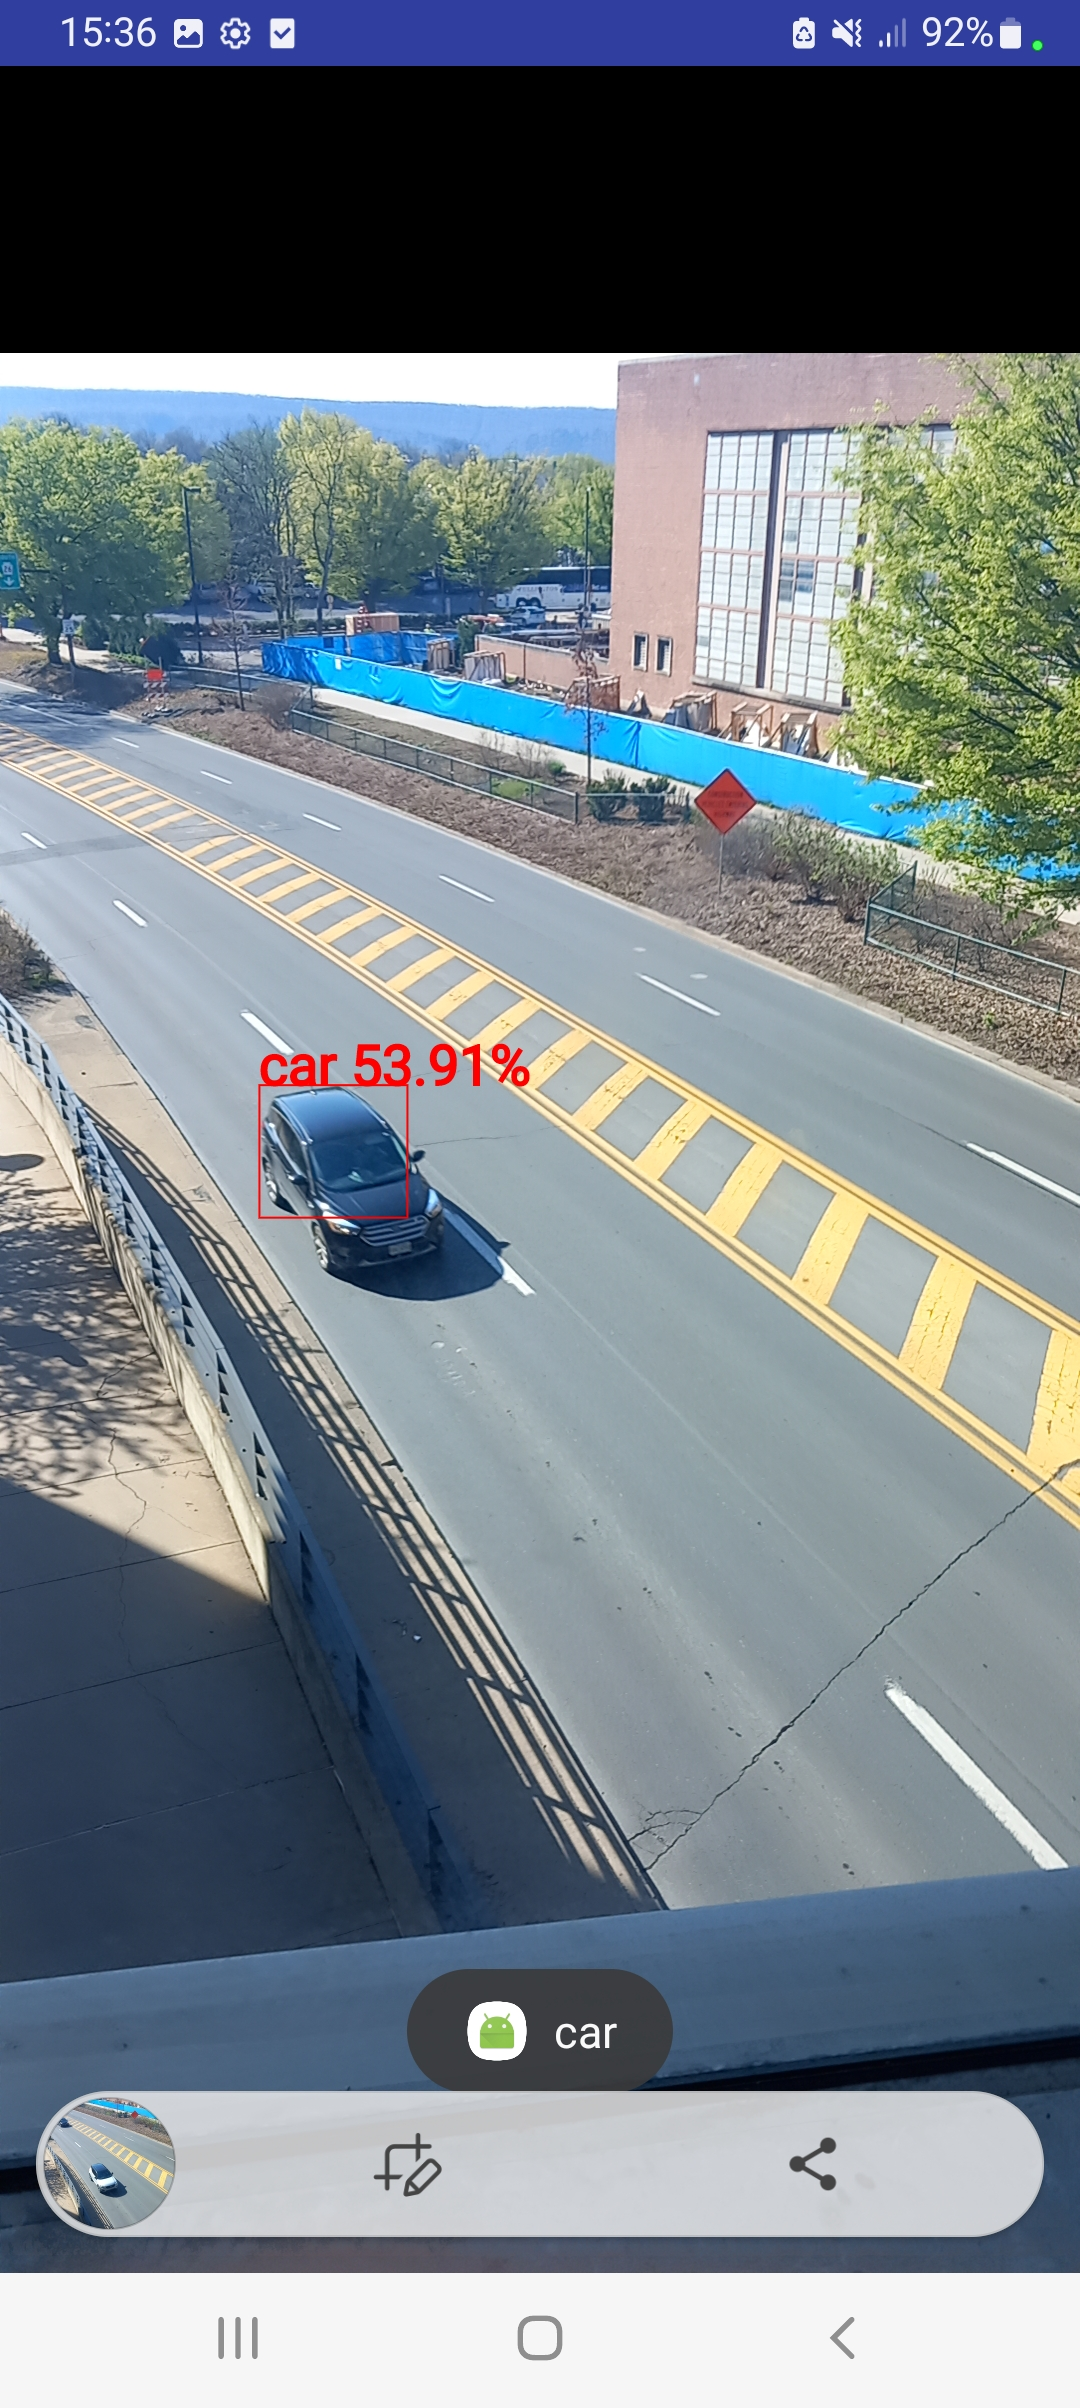
\includegraphics[scale=0.11]{figure/ObjectDetection_car.jpg}
    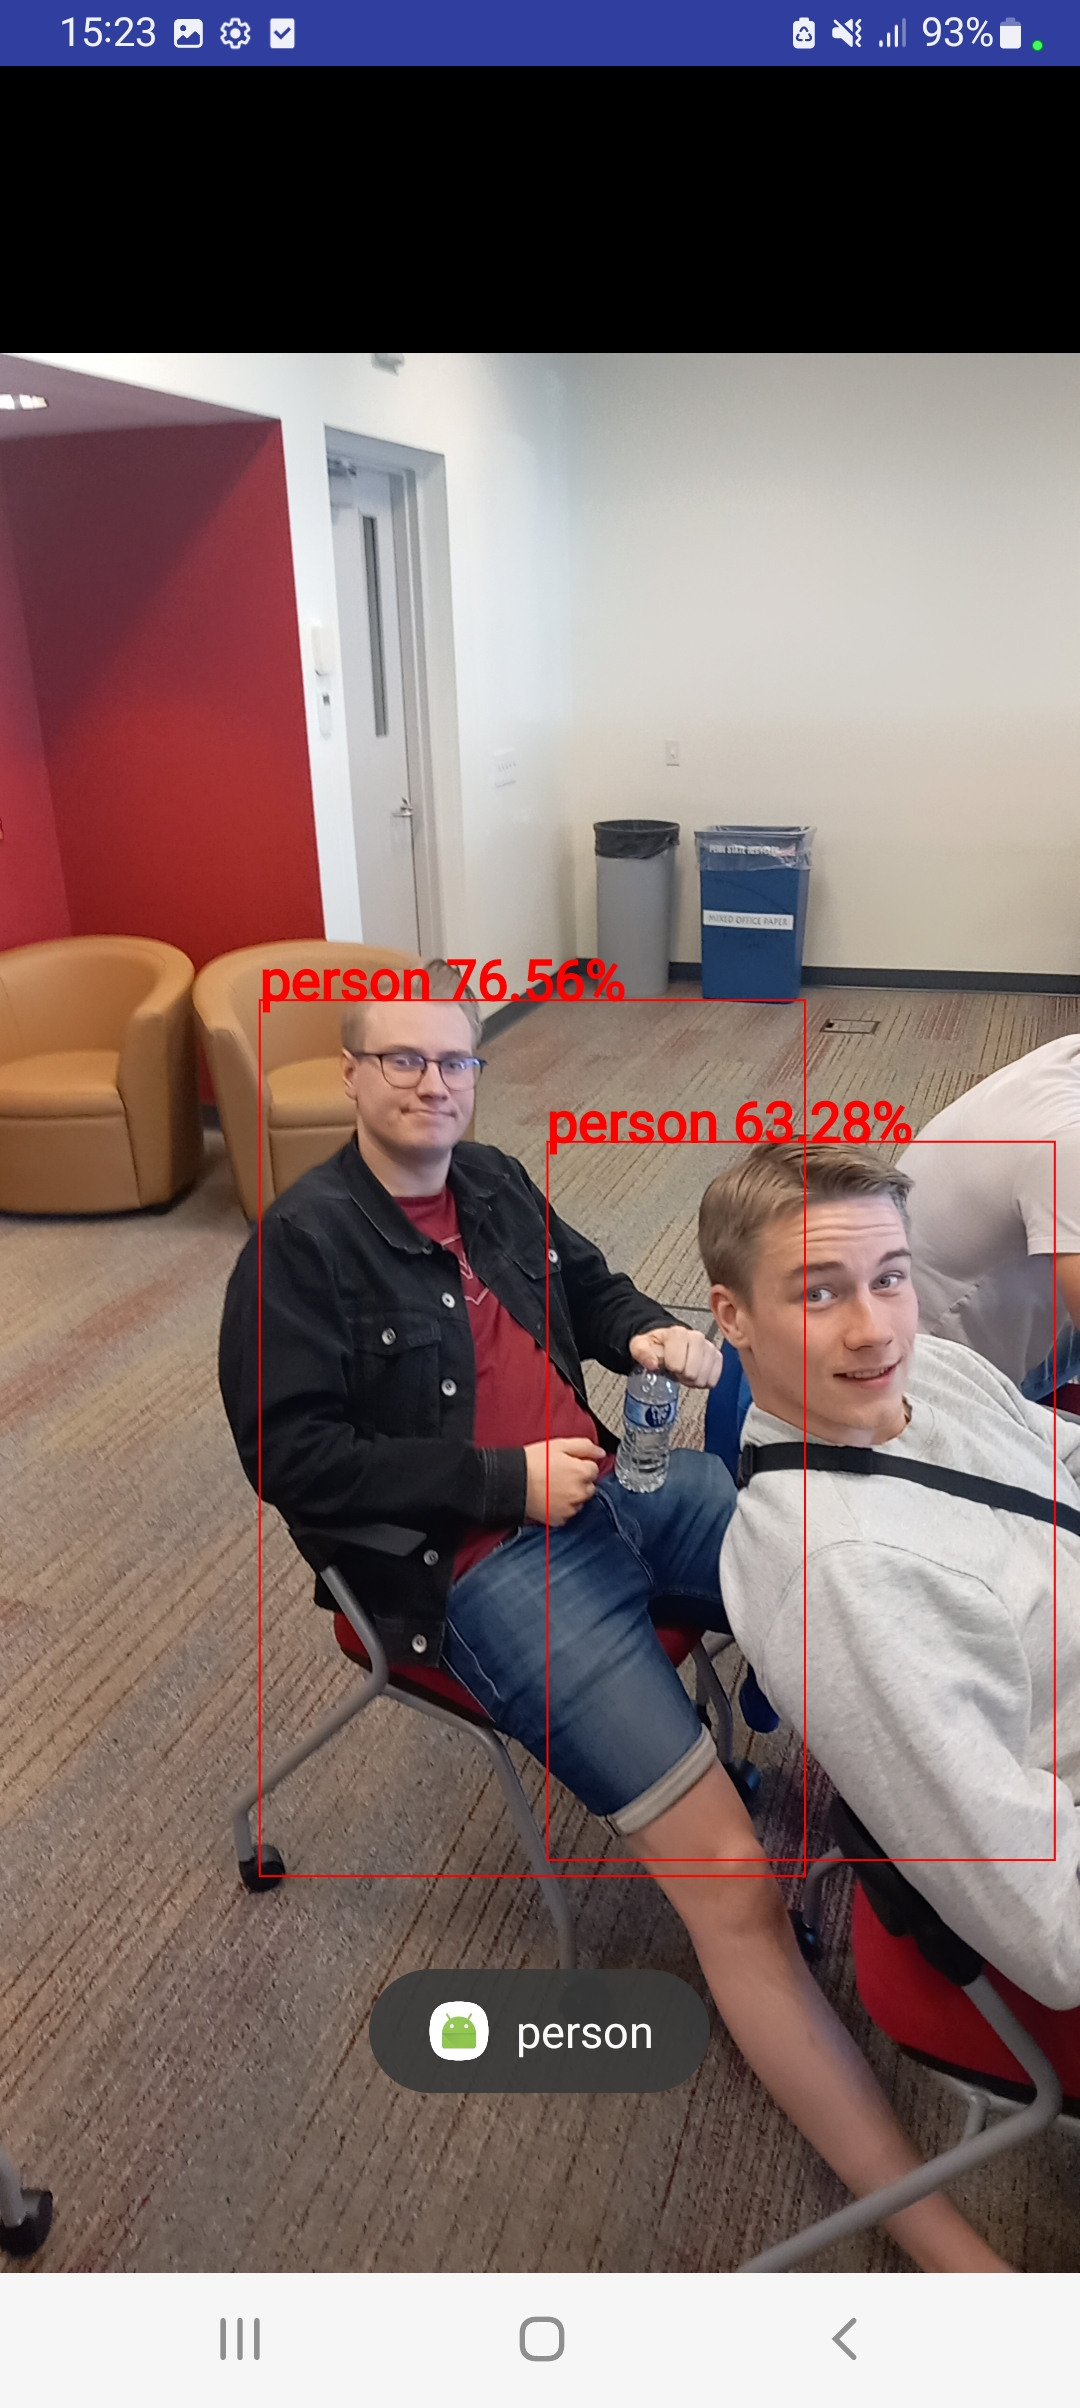
\includegraphics[scale=0.11]{figure/ObjectDetection_person.jpg}
    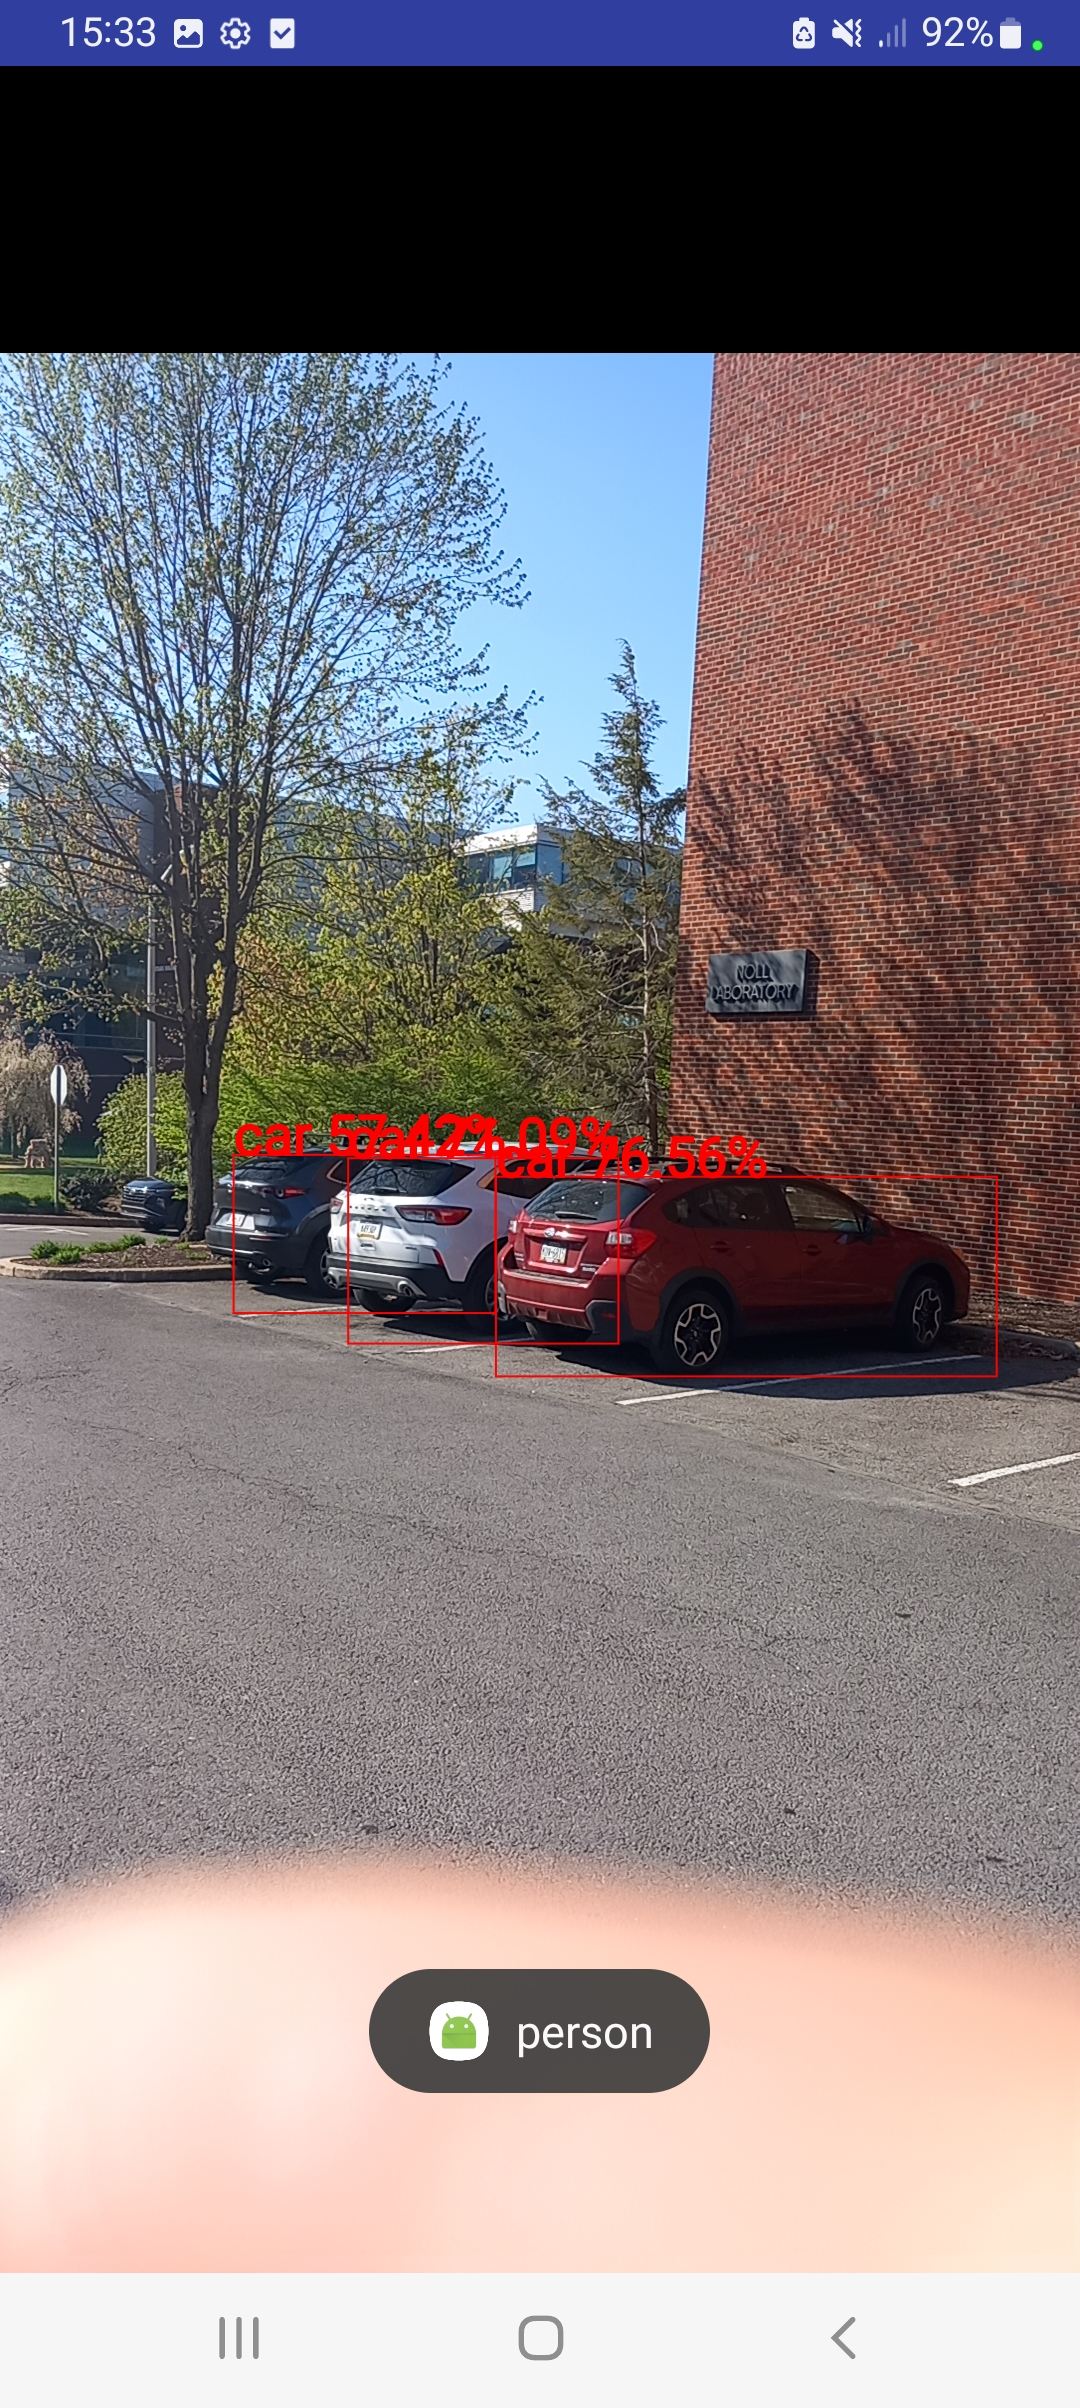
\includegraphics[scale=0.11]{figure/ObjectDetection_3cars.jpg}
    \caption{Screenshots from the mobile device. The pop up messages were not fully developed and are sometimes inaccurate. Source: Primary}
    \label{fig:Objectdetection-screenshot}
\end{figure}
\begin{figure}[H]
    \centering
    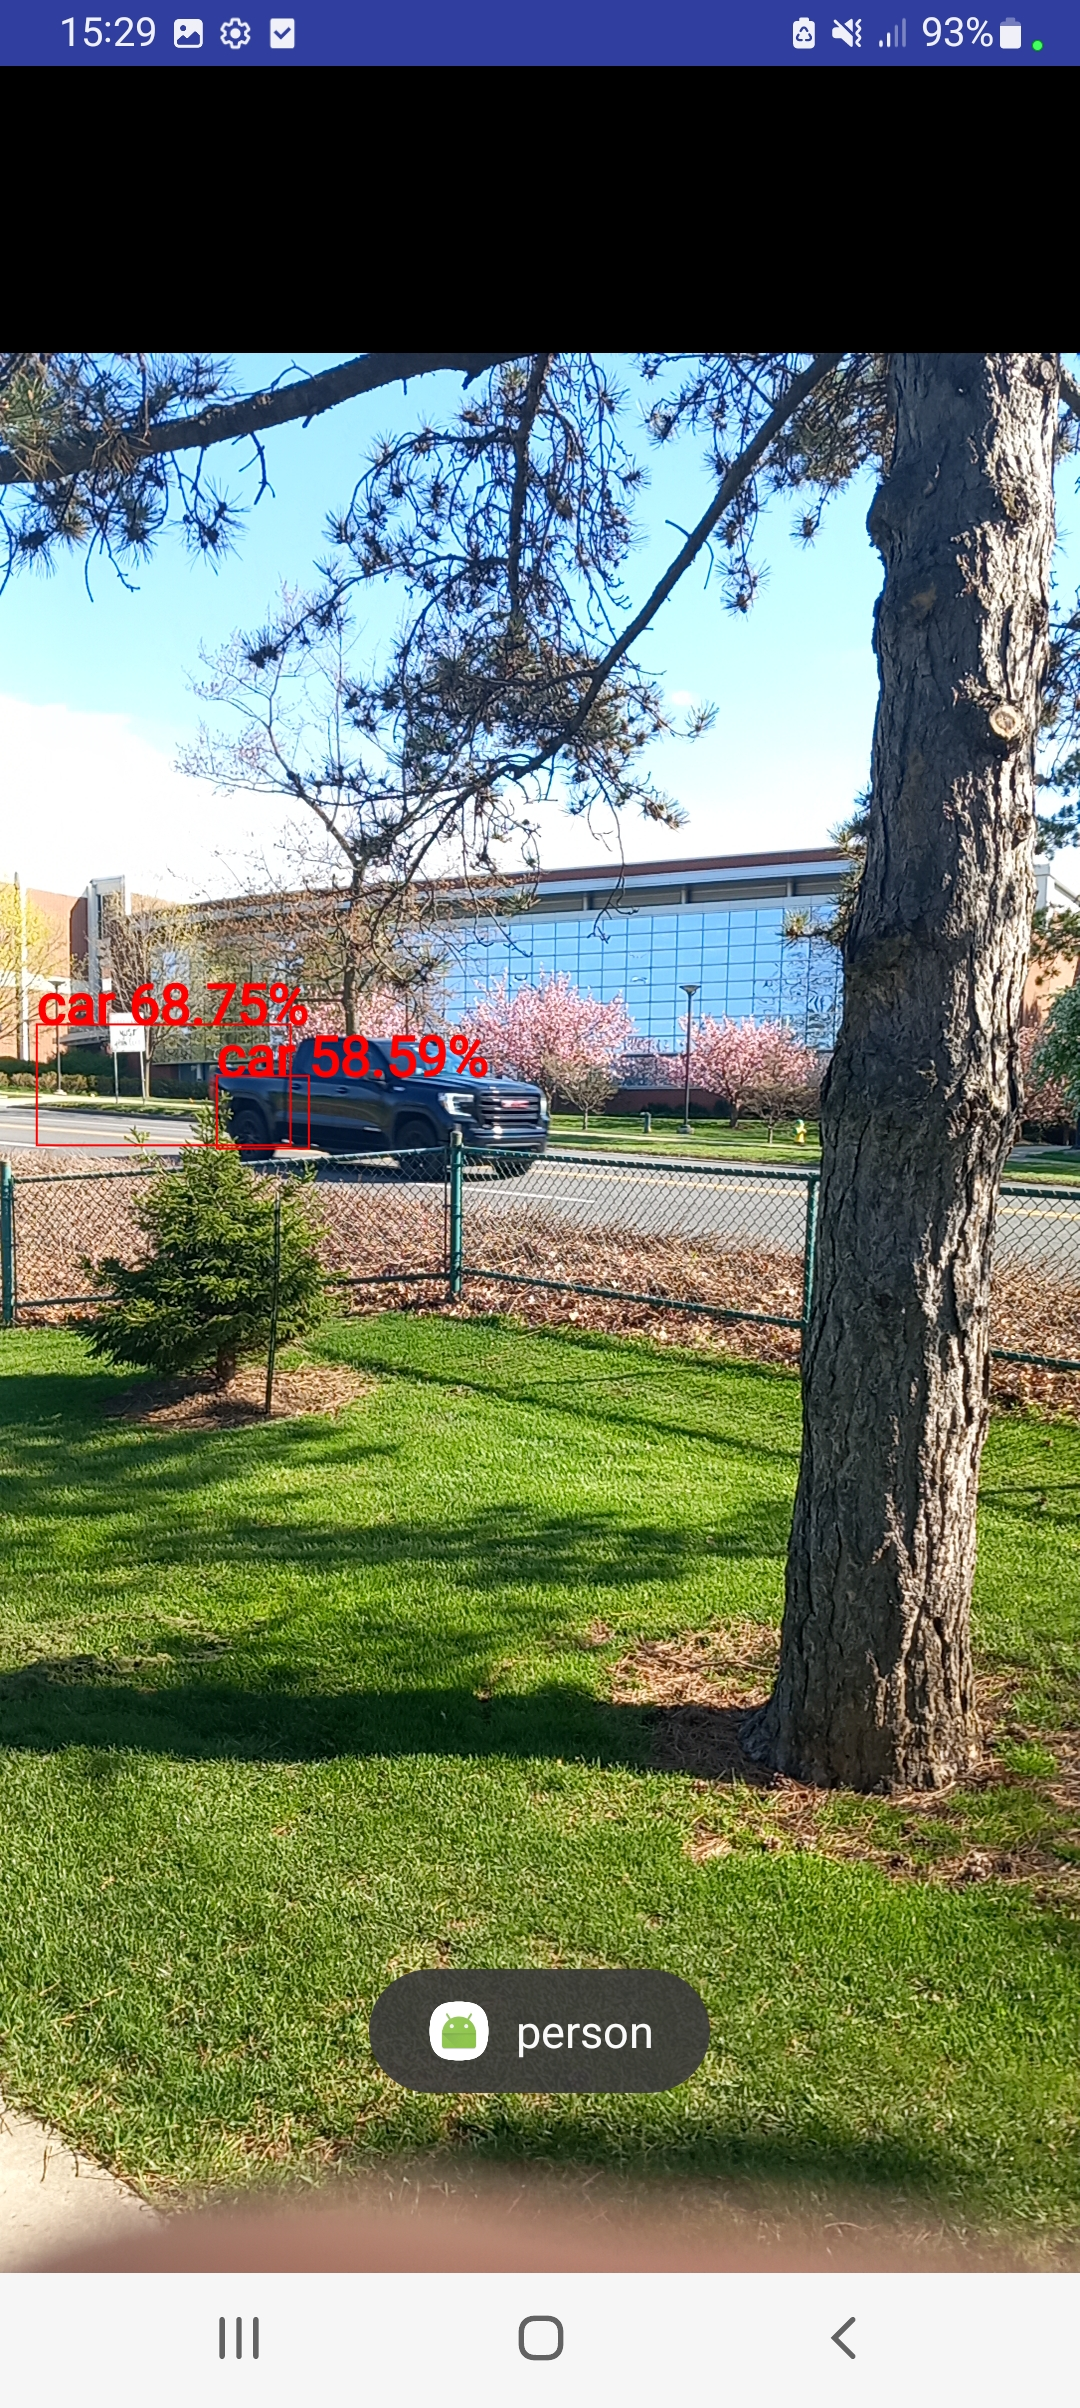
\includegraphics[scale=0.11]{figure/ObjectDetection_2in1.jpg}
    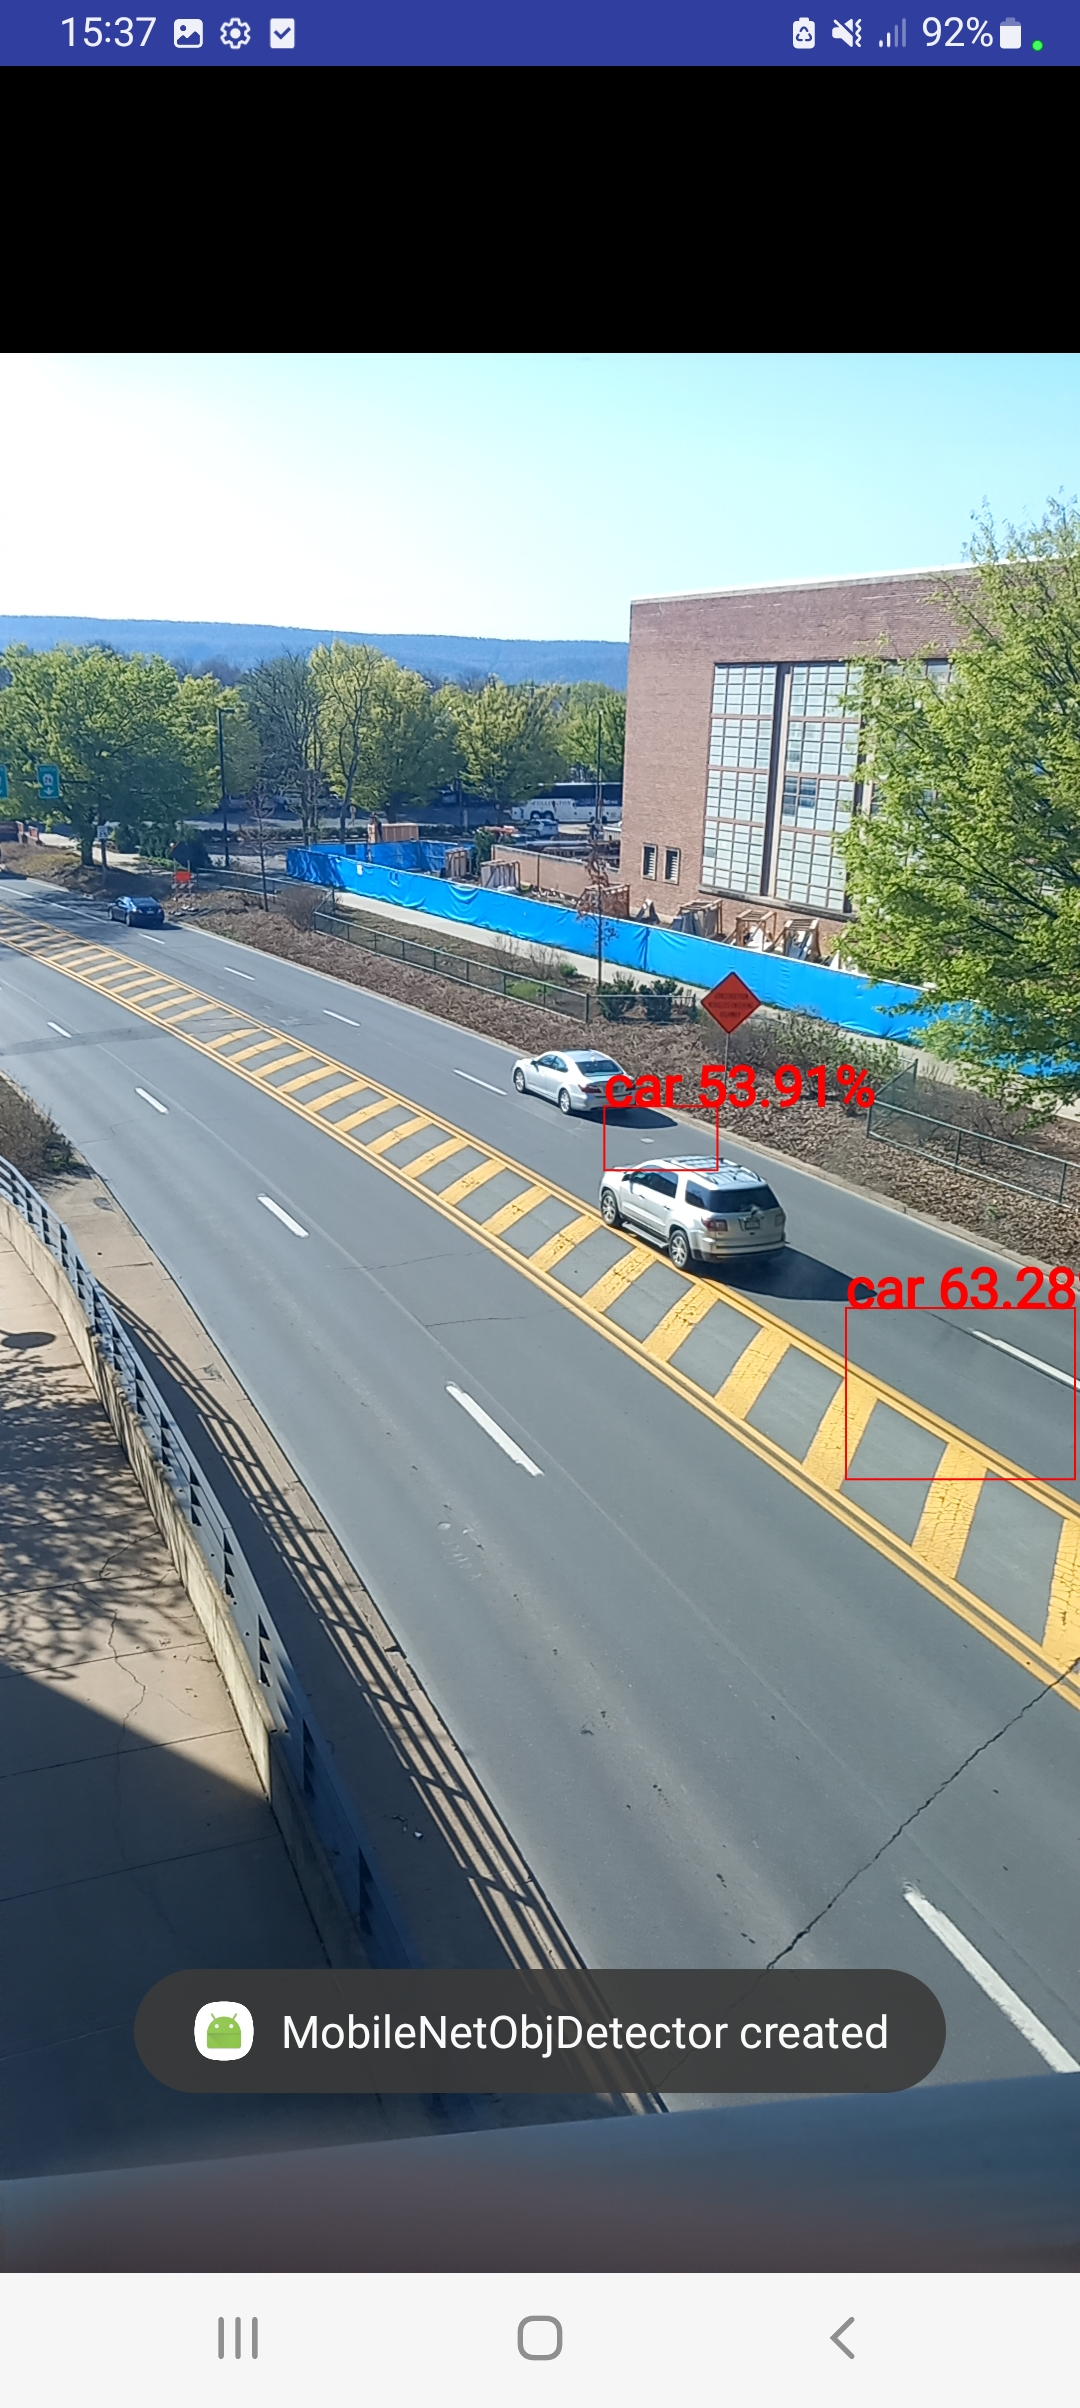
\includegraphics[scale=0.11]{figure/ObjectDetection_slow.jpg}
    
\includegraphics[scale=0.11]{figure/ObjectDetection_noFrame.jpg}
    \caption{Screenshots from the mobile device. The pop up messages were not fully developed and are sometimes inaccurate. Source: Primary}
    \label{fig:Objectdetection-screenshot2}
\end{figure}
Other tests, presented in Sec.~\ref{val_obj_det} were also conducted. The model was successful in detecting every non-moving car that it was tested on, an example is shown in Fig.~\ref{fig:Objectdetection-screenshot}. However, larger vehicles such as trucks, buses, and sometimes vans were not detected. This was expected since the model was designed to output only persons and cars. Next, moving cars and people was filmed, which revealed some limitations of the model. Although the model was able to handle moving objects, it struggled with certain scenarios. Fig.~\ref{fig:Objectdetection-screenshot2} shows the resulting issues. Finally, the model output frequency was tested to determine how often the model produced results to ensure that the model was quick enough for its intended use. The frequency and subsequent delay of the model can be seen in the picture in the middle of Fig.~\ref{fig:Objectdetection-screenshot2}. The model averaged four outputs per second. 
\\ \\
To implement the object detection algorithm using the drone's camera feed, it was first tested whether the gimbal on the drone could be controlled freely during a WaypointMission. This happened to be the case and the drone flew a simple WaypointMission while the gimbal was automatically controlled with predetermined movements.
\\ \\
Problems arised when trying to implement object detection on the drone camera. To process video and display it, the DJI SDK offers a class named DJICodecManager~\cite{DJIDJICodecManager} which offers relevant functions for video encoding and decoding. When trying to work with the DJICodecManager and pull live video data from the stream, the video was formatted in a YUV format~\cite{2019RGBDepacking}. YUV is an image format that separates the luminance (Y) component, representing brightness, from the chrominance components (U and V), representing color information. In this format, the Y, U, and V components are stored as three separate planes within a single array. The class was not able to display the video on screen while also feeding the camera feed to the object detection algorithm. An attempt to decode the YUV data and transform it to a format accepted by the object detection model was undertaken, without success. Following that the object detection on the drone camera was not implemented, the object tracking algorithm was put on hold until the issue was solved. 

\section{Cost-benefit analysis} \label{res:COSTBENEFIT}
As previously stated there was a requirement for conducting a cost-benefit analysis for the incorporation of the drones and the developed drone application. 
\\ \\
The current utilization of drones for filming the different tests at AstaZero’s facility is mostly stationary. The integration of the developed drone app, together with the existing software ATOS, will allow for dynamic filming. Whether the possibility of dynamic filming is beneficial, both from a financial standpoint and in terms of time however, is something that needs to be investigated. 
\\ \\
When conducting a cost-benefit analysis there are a lot of minor parameters which can be taken into account, and a lot of different viewpoints that could change depending on the chosen approach. This analysis is dissected into the major and more clearly stated points of affect. 
The main cost for the project would be the cost of (at least) one drone of type DJI Mavic Enterprise ZOOM, which is roughly 20000SEK~\cite{DJI_stockholm}.
\\ \\
However, depending on adopted approach, this expense could be considered a sunk cost, as the drones are already paid for, regardless of whether AstaZero chooses to utilize the project group's developed app or maintain the current configuration of stationary footage.
\\ \\
In addition, maintenance expenses such as unforeseen repairs and charging requirements should also be considered.
Furthermore there are the labor costs, information regarding how many workers are needed to conduct the tests are not specified and vary from time to time. However, a deduction of at least one manpower position is reasonable due to the app-enabled automatic flying capability of the drones, which eliminates the need for an individual human operator per drone, unlike the current configuration. However, considering that the development of the app is completely free for the client in terms of labor costs, the NPV-analysis will neglect salary costs for developers, making it non-applicable for use outside of this specific project.  
\\ \\
The implementation and subsequent development of the application will ensure the production of consistent and dynamic footage over an extended period of time. In the event that the trajectories for the test objects and the drones remain unchanged, this will establish standardized scenes for all future tests conducted. As a result, this will provide a clearer overview of the different tests and facilitate a more straightforward comparison of the various vehicles based on the footage.
\\ \\
Furthermore, if AstaZero chooses to continue to use DJI as their drone provider, and assuming that future versions of drones remain similar to the current models, the application will continue to serve as a useful tool for documentation of Euro NCAP tests without becoming obsolete. 
\\ \\
This configuration also reduces the need for human interaction, it also eliminates the risk for human errors while footage is being captured, making it feasible that the lifetime for the drones will be maximised. Combining all these considerations, the potential upside of this configuration heavily outweighs the minuscule potential downsides. 
\\ \\
In strictly monetary terms, the annual savings of the implementation can be calculated with data provided by the manager at the AstaZero facility through an interview. According to the facility-manager there are roughly 300 tests annually that includes the use of drones. The test itself in effective time takes five minutes, however, with estimated preparation-time it is rather around 15 minutes. The stated hourly cost for each worker was said to be 350 SEK. Taking these factors into consideration, the annual saved amount of the implementation totals to 26250 kr.
\\ \\
\subsection{Net present value analysis}
In order to quantify the costs and savings for implementing the drone configuration in monetary terms, there is a need to define the usual annual costs for the drones and for labor. AstaZero is an non-profit organization, which means that they are unlikely to have a discount rate for alternative investments. The NPV-analysis will therefore only take inflation into account when calculating the value. 
\\

All the data for the NPV-analysis are taken from an interview with the testing manager at the AstaZero facility. However, it is based on assumptions and is shown to give an overview for the monetary benefits of implementing the drone-app-configuration. The analysis is only taking 5 years into consideration, meaning that the net present value in fact could be a lot larger, provided that it does not become obsolete.

The following parameters are taken into consideration for the NPV:
\begin{itemize}
    \item Cost of one singular drone: 20000 SEK
    \item Saved amount annually for a reduction of one manpower: 26250 SEK
    \item Estimated annual maintenance costs: 1500 SEK
    \item Estimated future inflation rate: 4\% (which is way higher than the mean value over the last few decades, which is less than 2\%)
\end{itemize}
% Please add the following required packages to your document preamble:
% \usepackage[table,xcdraw]{xcolor}
% If you use beamer only pass "xcolor=table" option, i.e. \documentclass[xcolor=table]{beamer}
\begin{table}[h]
\caption{Five-year Net Present Value Analysis}
\begin{tabular}{|lcccccc|}
\hline
\rowcolor[HTML]{B6D7A8} 
\multicolumn{7}{|c|}{\cellcolor[HTML]{B6D7A8}\textbf{Net Present Value Analysis {[}SEK{]}}}                                                                                                                                                                                                                                                       \\ \hline
\multicolumn{1}{|l|}{Year}                                      & \multicolumn{1}{c|}{0}                              & \multicolumn{1}{c|}{1}                             & \multicolumn{1}{c|}{2}                             & \multicolumn{1}{c|}{3}                             & \multicolumn{1}{c|}{4}                             & 5     \\ \hline
\rowcolor[HTML]{A4C2F4} 
\multicolumn{1}{|l|}{\cellcolor[HTML]{A4C2F4}Drone investment}  & \multicolumn{1}{c|}{\cellcolor[HTML]{A4C2F4}-20000} & \multicolumn{1}{c|}{\cellcolor[HTML]{A4C2F4}}      & \multicolumn{1}{c|}{\cellcolor[HTML]{A4C2F4}}      & \multicolumn{1}{c|}{\cellcolor[HTML]{A4C2F4}}      & \multicolumn{1}{c|}{\cellcolor[HTML]{A4C2F4}}      &       \\ \hline
\multicolumn{1}{|l|}{Saved amount}                              & \multicolumn{1}{c|}{}                               & \multicolumn{1}{c|}{26250}                         & \multicolumn{1}{c|}{26250}                         & \multicolumn{1}{c|}{26250}                         & \multicolumn{1}{c|}{26250}                         & 26250 \\ \hline
\rowcolor[HTML]{A4C2F4} 
\multicolumn{1}{|l|}{\cellcolor[HTML]{A4C2F4}Maintenance costs} & \multicolumn{1}{c|}{\cellcolor[HTML]{A4C2F4}}       & \multicolumn{1}{c|}{\cellcolor[HTML]{A4C2F4}-1500} & \multicolumn{1}{c|}{\cellcolor[HTML]{A4C2F4}-1500} & \multicolumn{1}{c|}{\cellcolor[HTML]{A4C2F4}-1500} & \multicolumn{1}{c|}{\cellcolor[HTML]{A4C2F4}-1500} & -1500 \\ \hline
\multicolumn{1}{|l|}{Net value (NV)}                            & \multicolumn{1}{c|}{}                               & \multicolumn{1}{c|}{24750}                         & \multicolumn{1}{c|}{24750}                         & \multicolumn{1}{c|}{24750}                         & \multicolumn{1}{c|}{24750}                         & 24750 \\ \hline
\rowcolor[HTML]{A4C2F4} 
\multicolumn{1}{|l|}{\cellcolor[HTML]{A4C2F4}Inflation rate}    & \multicolumn{1}{l|}{\cellcolor[HTML]{A4C2F4}}       & \multicolumn{1}{c|}{\cellcolor[HTML]{A4C2F4}4\%}   & \multicolumn{1}{c|}{\cellcolor[HTML]{A4C2F4}4\%}   & \multicolumn{1}{c|}{\cellcolor[HTML]{A4C2F4}4\%}   & \multicolumn{1}{c|}{\cellcolor[HTML]{A4C2F4}4\%}   & 4\%   \\ \hline
\multicolumn{1}{|l|}{NV adjusted for inflation}                 & \multicolumn{1}{c|}{-20000}                         & \multicolumn{1}{c|}{23798}                         & \multicolumn{1}{c|}{22883}                         & \multicolumn{1}{c|}{22003}                         & \multicolumn{1}{c|}{21156}                         & 20343 \\ \hline
\rowcolor[HTML]{B6D7A8} 
\multicolumn{7}{|c|}{\cellcolor[HTML]{B6D7A8}Net present value = $\sum$ NV = 90183 kr}                                                                                                                                                                                                                                                              \\ \hline
\end{tabular}
\end{table}





